
\documentclass{jpp}
\usepackage{graphicx}
% \usepackage{epstopdf, epsfig}
\graphicspath{.}
\usepackage[german]{babel}
\usepackage{hyperref} 
\usepackage{amsmath}
\usepackage{blindtext}
\usepackage{titlesec}
\title{Das Meistern von chinesischem Schach mit autodidaktischem Reinforcement Learning}

\author{Simon Ma (15)\aff{1}
  \corresp{\email{simon.mama07@gmail.com}}
  }

\affiliation{\aff{1}Schillerschule Hannover,
Ebellstr. 15, 30629 Hannover, Germany}


\begin{document}
\begin{figure}
\centering

\includegraphics[width={0.5\textwidth}]{loogo.png}
\end{figure}
\maketitle


Projektbetreuerin: Birgit Ziegenmeyer

Institution: Schillerschule Hannover

Thema des Projektes:

Die Entwicklung eines autodidaktischen Reinforcement Learning 

Algorithmus erweitert mit einem hochperformanten Suchalgorithmus 

um chinesisches Schach zu meistern

Fachgebiet: Mathematik/Informatik

Wettbewerbssparte: Jugend forscht

Bundesland: Niedersachsen

Wettbewerbsjahr: 2023

\newpage

\tableofcontents

\newpage

\section{Kurzfassung}
Xiangqi, chinesisches Schach, ist ein unvorstellbar komplexes Spiel, dessen Meisterung Jahrzehnte dauert - für einen Menschen. 
CheapChess ist meine Xiangqi Computer-Applikation, mit Fokus auf einer selbstlernenden KI, die sich um die Frage dreht, wie sich die ressourcenintensiven existierenden Programme optimieren und sich komplexe Probleme kostengünstig lösen lassen.
Zentrale Schwerpunkte lagen neben der Entwicklung einer Xiangqi-Applikation vor allem auf dem Entwurf und der Optimierung eines Reinforcement Learning Algorithmus, der ein Convolutional Neural Network nur durch simulierte Spiele gegen sich selbst trainiert. Seine Entscheidungen werden analysiert und ggf. korrigiert, wofür ich einen hochperformanten Such-Algorithmus entwickelte. So erreichte ich eine Reduktion der benötigten Hardware um $500.000\%$, entwarf dafür neue Konzepte und es entstand ein flexibler, starker Spieler.
\section{Einleitung}\label{sec:einleitung}
Bereits für die Väter der Informatik wurde Computer Schach zur Herausforderung. Babbage, Turing, Shannon und von Neumann entwickelten schon in den frühen 1950ern Algorithmen und Hardware, um mehr Verständnis über die Domäne zu erlangen. Schach wurde schnell zur größten Herausforderung für Generationen von Informatikern und Forschern der künstlichen Intelligenz. 

Die meisten Schach-Programme, z.B. Stockfish, basieren dabei auf einer Kombination von hocheffizienten Suchalgorithmen, domänenspezifischen Optimierungen und handgefertigten Evaluationsfunktionen, welche Jahre lang von Experten optimiert wurden. 

Mit Deepminds AlphaZero führten 2017 innovative Konzepte und scheinbar unendliche Ressourcen zu einem der größten Durchbrüche in der KI-Forschung. Denn anstelle der herkömmlichen Methoden lernte ein Convolutional Neural Network (CNN) mithilfe eines raffinierten Reinforcement Learning allein durch Spiele gegen sich selbst Schach, Shogi und Go und schlug in jedem Spiel den jeweilige Weltmeister. Nur ist das Programm nicht öffentlich zugänglich und wohl kaum jemand besitzt die 5000+ Tensor Processing Units (TPUs), die Deepmind zur Verfügung standen. 

Das grundsätzliche Ziel von CheapChess ist die Anpassung benötigter Ressourcen auf normale Konsumenten und die Förderung von Zugänglichkeit zu innovativen Konzepten wie AlphaZero. Anders als Stockfish und AlphaZero fokussiere ich mich dabei jedoch spezifisch auf Xiangqi (chinesisches Schach). Xiangqi erfordert wegen seiner extremen Komplexität besondere Achtung auf Effizienz und durfte noch keine intensive Forschung genießen.

So entwarf ich eine Python Xiangqi Applikation und entwickelte einen effizienten autodidaktischen Reinforcement Learning Algorithmus ergänzt von hochoptimierten Such-Algorithmen. Es entstand eine Kombination aus den innovativen Konzepten von AlphaZero und den traditionellen Methoden von Stockfish, die beim Training beobachtet und zum Spielen herausgefordert werden kann. 

Meine Arbeit soll einerseits eine radikale Reduktion der benötigten Hardware ermöglichen, andererseits den Stärken einer Methode erlauben, für die Schwächen der anderen zu kompensieren und darüber hinaus zu neuen Einblicken in die taktische Welt von Xiangqi führen.

\section{Einführung zu Xiangqi}
Xiangqi, auch bekannt als chinesisches Schach, ist ein strategisches Brettspiel, das in China sehr beliebt ist. Es ist in einigen Aspekten ähnlich wie Schach, weist aber auch Unterschiede auf. So wird es auf einem $9 \cdot 10$ Brett gespielt und es gibt andere Figuren.

\begin{figure}
  \centering
  \begin{minipage}[b]{0.49\textwidth}
    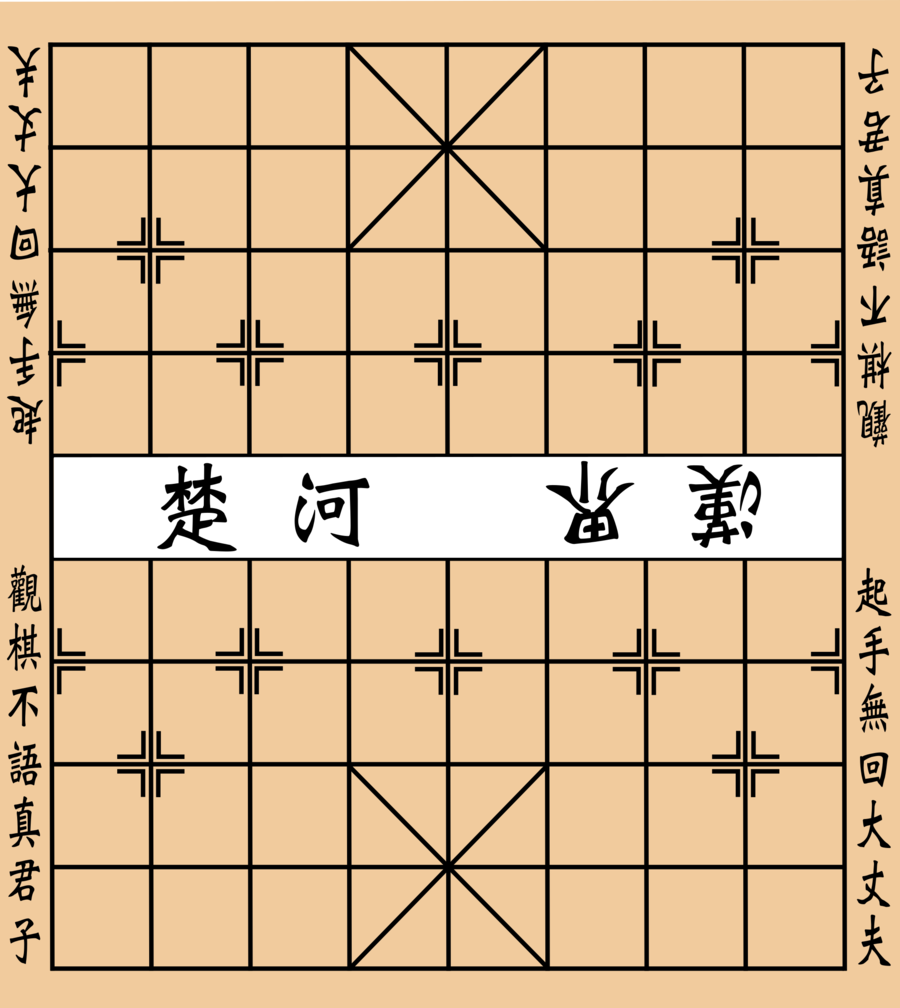
\includegraphics[width=\textwidth]{board.png}
    \caption{Die Standardaufstellung eines Xiangqi-Spiels, veranschaulicht mit dem GUI meiner Applikation}
    \label{fig:board}
  \end{minipage}
  \hfill
  \begin{minipage}[b]{0.49\textwidth}
    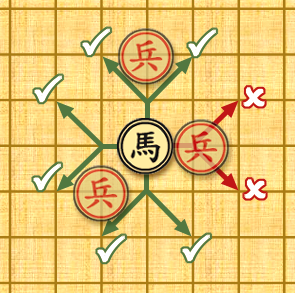
\includegraphics[width=\textwidth]{MovementOfHorsePiece.png}
    \caption{Züge des Pferdes}
    \label{fig:Horse}
  \end{minipage}
\end{figure}
Das Brett besteht aus $9 \cdot 10$ Linien und Figuren stehen auf den Kreuzungen dieser Linien statt auf den Feldern. In der Mitte des Bretts zwischen Reihe fünf und sechs befindet sich der Fluss, also die Grenze der beiden Reiche und um den König herum ein Palast, welcher mit zusätzlichen Linien markiert ist \ref{fig:board}.


Der Feldherr / König geht immer nur einen Schritt waagerecht oder senkrecht. Er darf den Palast nie verlassen, kann insgesamt also nur neun Felder betreten. Eine Rochade gibt es nicht. Die beiden gegnerischen Feldherren dürfen sich niemals ohne einen dazwischen stehenden Stein auf einer Linie gegenüberstehen. Der „Todesblick“ der Feldherrn verbietet dies, was besonders im Endspiel genutzt werden kann, um ein Patt (das im Xiangqi kein Remis, sondern ein Sieg ist) zu erzwingen.

Die Leibwächter / Berater gehen immer nur einen Schritt diagonal auf ein unmittelbar benachbartes Feld und dürfen den Palast ebenfalls nicht verlassen. Somit stehen beiden zusammen nur fünf Felder zur Verfügung, nämlich die Palastmitte und dessen vier Ecken.

Die Elefanten gehen genau zwei Schritte in diagonaler Richtung. Falls das zwischenliegende (übersprungene) Feld besetzt ist, wird der Zug geblockt. Darüber hinaus dürfen die Elefanten niemals den Fluss überqueren.

Die Pferde entsprechen im Wesentlichen den Springern des internationalen Schachs, können jedoch ebenfalls blockiert werden. Ein Pferd bewegt sich in seinem Zug in zwei Schritten: zuerst ein Feld waagerecht oder senkrecht in beliebiger Richtung und anschließend ein Feld diagonal. Das Pferd wird blockiert, wenn eine andere Figur auf dem zuerst zu betretenden Feld steht \ref{fig:Horse}.

 Der Turm / Wagen entspricht der den Türmen des europäischen Schachs. 
 
 Die Kanonen gibt es in internationalem Schach nicht. Wenn sie nicht schlagen, bewegen sie sich wie der Wagen. Zum Schlagen muss sich irgendwo zwischen dem gegnerischen Stein, und der Kanone genau ein anderer Stein befinden (Schanzenstein), der beim Schlagen übersprungen wird.
 
 Die Soldaten / Bauer bewegen sich ein Feld nach vorne und können nicht zurückgehen. Anders als Bauer im internationalen Schach können sie aber nach Überquerung des Flusses ein Feld seitlich ziehen und schlagen nicht diagonal, sondern im herkömmlichen Zugmuster (senk- und waagerecht)
 
\section{Methoden}
\begin{figure}
    \centering
    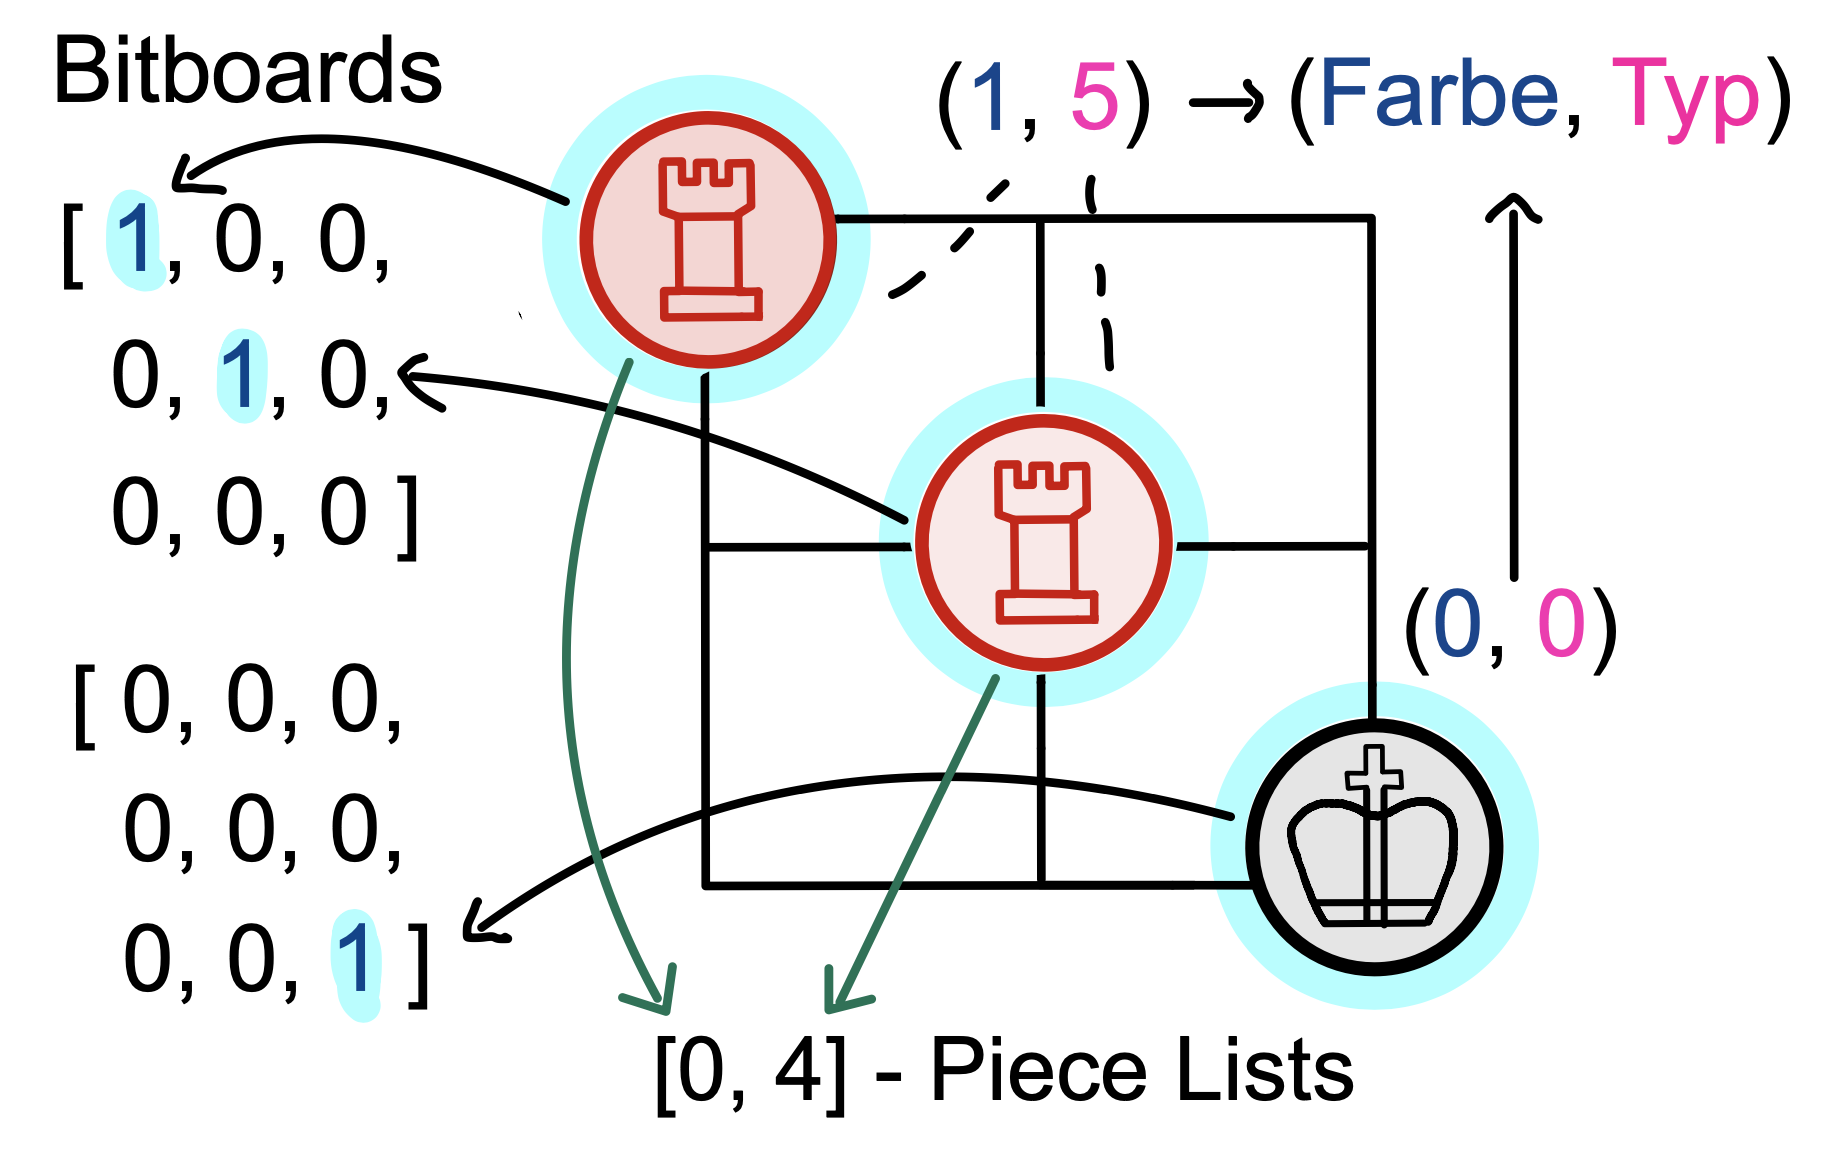
\includegraphics[width={0.6\textwidth}]{Board repr.png}
    \caption{Simplifizierte Visualisierung der internen Brettrepräsentation}
    \label{fig:repr}
\end{figure}
\subsection{interne Brettdarstellung}
Die Figuren werden als Tupel repräsentiert, wobei Index 0 die Farbe und Index 1 den Typ bestimmt. Die darstellung als 8-bit Zahl funktionierte, wies sich aber als deutlich langsamer auf. Das Brett ($9\cdot10$) wird in drei verschiedenen Weisen dargestellt:

\begin{enumerate}
\item Feldzentrisch als ein-dimensionale Liste mit 90 Stellen, 0 für leeres Feld, Tupel für Figur
\item Figurenzentrisch als drei-dimensionale Liste der besetzten Felder für jeden Figurentyp jeder Farbe. \ref{fig:repr} Form: $(2 \cdot 7 \cdot n)$ wobei $n$ die variierende Anzahl des Figurentypes im Verlauf des Spiels ist (Hier ist $n = 2$). diese Listen werden genutzt, um schnell auf die besetzen Felder eines Figurentyps zuzugreifen.
\item drei-dimensionales array von Bitboards für jeden Figurentyp jeder Farbe. Form: $(2\cdot7\cdot90)$. Bitboards sind binäre Repräsentationen des Bretts wo eine 0 für ein leeres und eine 1 für ein besetzt Feld steht \ref{fig:repr}. Ich nutze sie als Eingabe für mein Neuronales Netzwerk.
\end{enumerate}

\subsection{Schwerpunkt: Zuggeneration}
Die Zuggeneration ist die effiziente Übersetzung der Spielregeln in Code, baut das Fundament für jedes Spiel und wird innerhalb der KI Milliarden Male genutzt. Darum ist exzellente Performance essenziell. Da keine gute Python-Implementationen existieren, schrieb ich meine eigene, bestehend aus zwei Hauptkomponenten:
\begin{enumerate}
    \item Pseudo-erlaubte Zuggeneration / Precomputed move maps, Kodierung von Bewegungsmustern ohne Analyse der Legalität
    \item Generation erlaubter Züge, dynamischer Legalitätsfilter
\end{enumerate}
\subsubsection{Generation pseudo-legaler Zugmuster}
In der ersten Komponente werden sogenannte Move-Maps generiert, worin die grundsätzlichen Zugregeln kodiert sind.  Diese Züge können in bestimmten Situationen aber gegen die Regeln verstoßen, weshalb sie nur \textit{pesudo-legal} sind. Die Generation ist einmalig, weshalb die Peformance hier nicht ausschlaggebend ist.

Ich überlegte mir: Da das Brett eine ein-dimensionale Repräsentation besitzt, kann ein Skalar-Offset (ein-dimesionaler Wert)  genutzt werden, um zu einem anderen Feld zu gelangen. Für einen Schritt nach Osten wäre dieser z.B. 1, nach Norden -9, nach Nord-Osten -8. Aus diesen Offsets berechne ich dann die jeweiligen Pferd-Sprünge und füge all diese einer Offset-Liste hinzu. Diese stehen immer in der gleichen Reihenfolge und können mit einem Richtungsindex in Bezug genommen werden. offsets[0] ist z.B. -9 (Norden)

Die Move-Map der Kanone und des Turms besteht hierbei aus einer Liste an Hash-Tabellen, wo der Listen-Index für das Feld steht und der  Hash-Schlüssel den Richtungsindex angibt. Dafür wird für jedes Feld und für jede Richtung (N, O, S, W; Richtungsindex 0 - 3) die Distanz zum Ende des Bretts berechnet, dann die Anzahl von Schritten in die jeweilige Richtung gegangen und alle Felder auf dem Weg als Ziel für den jeweiligen Richtungsindex hinzugefügt.

Für das Pferd werden die vorher berechneten Pferd-Sprung-Offsets genutzt. Die Manhattan Distanz zwischen Start und Ziel muss exakt drei betragen um Sprünge zur anderen Seite des Bretts zu vermeiden. Da das Brett 1D ist, würde (9, 16) trotz eines validen Offsets zur anderen Seite des Bretts Springen, was nicht erlaubt ist.

Die Elefanten Move Map wird mit einem Depth-First-Search (DFS) Algorithmus generiert, da kein einfaches Muster zwischen den erreichbaren Feldern besteht. Hierfür nutze ich ein Stack $s$ und füge ein Start-Feld hinzu. Nun wird iterativ von $s$ ein besuchtes Feld $f$ entfernt und für dieses alle möglichen Ziele $z$ an $s$ angehängt. Währenddessen wird die Move Map an Hash-Schlüssel $f$ mit $z$ ergänzt. Dabei kann kein Ziel $z_i$ seinen Ursprung $f_i$ zu $s$ hinzufügen. Das gleiche Prinzip wie bei dem Pferd gilt für den Elefanten, um unerlaubte Sprünge zu vermeiden.

Für die Leibwächter wird jeweils das Zentrum $c$ des Palastes ausgewählt und ein Schritt diagonal in die Ecken $e$ des Palastes gegangen. Für jede Ecke wird der Move-Map an Hash-Schlüssel $c$ das Ziel $e_i$ und an Hash-Schlüssel $e_i$ das Ziel $c$ hinzugefügt.

Für den König / General berechne ich die möglichen vertikalen Offsets für die drei Reihen und die horizontalen Offsets für die drei Spalten im Palast. Diese werden dann zu einem zweidimensionalen Offset-Vektor für alle neun Felder im Palast kombiniert und daraus die möglichen Züge berechnet. 

Der Handlungsraum (en. Action Space) umfasst alle möglichen Züge.

\subsubsection{ Generation erlaubter Züge}
Dieser Komponent ist ein Filter, um unerlaubte Züge zu erkennen und zu entfernen. Er umfasst im Quellcode mehr als 800 Zeilen und würde für eine genaue Erklärung alleine schon 15 Seiten erfordern, weshalb ich diesen Teil abstrahiert erklären muss.

Der erste Gedanke war es, für jeden Zug alle möglichen Antworten des Gegners zu generieren. Wenn eine Antwort davon den König schlägt, ist der Zug unerlaubt. Das Problem ist hierbei aber nicht nur die unglaubliche Ineffizienz, sondern vor allem die Ungenauigkeit - Was ist, wenn diese Antwort selber unerlaubt ist? 

Da diese Komponente essenziell für die Performance aller folgenden Algorithmen ist und keinen Spielraum für Ungenauigkeiten bietet, ist dies keine Lösung.

So entwickelte ich einen Algorithmus, um Angriffsdaten zu generieren und mithilfe dieser die (un-) erlaubten Züge zu erkennen.
Es müssen dafür Bedrohungen und gepinnte Figuren erkannt und das Verhalten dieser Figuren unterschiedlich angepasst werden. Offensive Figuren, mögliche Bedrohungen müssen identifiziert werden um unnötige Angriffsdaten-Generation zu vermeiden.
Diese Grundidee dieser Komponente besteht also aus drei Teilen:
\begin{itemize}
    \item mögliche Bedrohungen erkennen
    \item Angriffsdaten generieren
    \item mit den Angriffsdaten unerlaubte Züge herausfiltern
\end{itemize}

Besondere Schwierigkeiten bereitete mir dabei die Kanone, da sie für äußerst skurrile Grenzfälle sorgen kann, mit denen ich vorher nicht gerechnet hatte und die sich nur durch unerwartetes Verhalten des Programms und viel Troubleshooting identifizieren und lösen ließen.

Die Performance vom Zugfilter verbesserte sich mit jeder Optimierung. Diese bestanden grundsätzlich immer aus der Integration von neuen Ideen und der geschickten Veränderung von Datenstrukturen oder vom Algorithmus.

\subsection{Alpha-Beta-Suche}
Die Suche in einer KI beschreibt den Prozess, unterschiedliche Züge zu spielen, diese zu bewerten und aus ihnen den besten Zug zu wählen. Hierfür hilft es, sich das Spiel als einen Baum mit Spielsituationen {$s_{root}, s_2, s_3 ...$} als Knoten vorzustellen. Diese Knoten werden von Zügen {$a_1, a_2, a_3 ...$} als Zweige verbunden. Hierbei ist $s_{root}$ der Startzustand und alle untergeordneten Knoten beschreiben Positionen, die aus Folge von diesen Zügen entstehen. Diese Baum Datenstruktur wird auch \textit{Search Tree} bzw. \textit{Such-Baum} genannt. 
Wenn das Endergebnis des Spiels für jeden Zug kennen würden, bestünden die Bewertungen nur aus Verlust, Unentschieden und Sieg und die KI müsste nur einen Zug in die Zukunft schauen, um den Besten zu finden. In der Praxis ist kann jedoch aufgrund der unvorstellbar großen Such-Baum-Komplexität von Xiangqi ($10^{150}$) der exakte Wert einer Position nicht ermittelt werden, weshalb dieser geschätzt werden muss.
\subsubsection{Standard-Heuristic-Evaluation-Function (SHEF)}
Die \textit{Standard-Heuristic-Evaluation-Function} ist eine \textit{Hand-Crafted-Evaluation (HCE)}, die genau dafür genutzt wird, indem sie einen statischen Wert für jede Figur festlegt \ref{fig:wert}.
\textit{Piece-Square-Tables} werden genutzt, um diese Werte zu spezifizieren. Diese gehen von der Beobachtung aus, dass Figuren abhängig von ihrer Position unterschiedlich stark sind und geben demnach jeder Figur einen Feld-spezifischen Wert. Beispielsweise ist ein Turm vor dem gegnerischen Palast stärker als in einer Ecke.
\begin{figure}
\centering
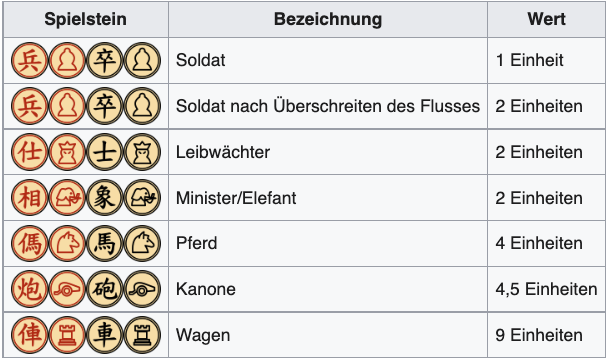
\includegraphics[width={0.6\textwidth}]{Wert.png}
\caption{Wert der Figuren}
\label{fig:wert}
\end{figure}

\subsubsection{MiniMax}
Es wird angenommen, dass jeder Spieler an jeder Situation den optimalen Zug spielt, dessen resultierende Spielsituation laut der SHEF seinen erwarteten Gewinn maximiert und jeder Gegner versucht, diesen zu minimieren. So werden die Blätter (unterste Knoten) des Such-Baums mit den Evaluationen der jeweiligen Positionen gekennzeichnet und die restlichen Knoten werden rekursiv durch Auswahl des Zuges mit dem höchsten (für \textbf{max}) bzw. dem niedrigsten (für \textbf{min}) Gewinn gekennzeichnet. Ich habe eine elegantere Methode genutzt, wo jeder Spieler den negativen Wert seiner besten Evaluation an den Elternknoten (Gegner) weitergibt, denn der beste Wert für einen Spieler ist der schlechteste Wert für seinen Gegner. Somit kann auf unterschiedliche Operationen basierend auf dem Spieler verzichtet und immer die \textit{max()} Funktion genutzt werden.

Ich implementierte diesen Algorithmus, erzielte jedoch nicht mein Ziel, hochperformante Algorithmen zu schreiben. Die Suche dauerte schon für drei Züge in die Zukunft rund zwanzig Sekunden. Dies lag daran, dass Minimax-Algorithmen eine exponentielle Zeit-Komplexität von $O(b^d)$ haben, wobei $b$ der Ausdehnungsfaktor und $d$ die Tiefe (en. depth) der Suche ist.
\subsubsection{Alpha-Beta-Pruning}
Ich fand heraus, dass Alpha-Beta-Pruning die Leistung des Minimax-Algorithmus deutlich verbessert, indem es unbrauchbare Zweige des Such-Baumes frühzeitig abschneidet. Dies wird erreicht, indem für jeden Knoten im Baum zwei Werte, $\alpha$ und $\beta$, verwendet werden. $\alpha$ repräsentiert den besten Wert, den der aktuelle Spieler erreichen kann, und $\beta$ repräsentiert den besten Wert, den der gegnerische Spieler erreichen kann. Wenn $\alpha \geq \beta$ ist, wird der Rest des Zweigs abgeschnitten, da der aktuelle Spieler keine Möglichkeit hat, ein besseres Ergebnis zu erzielen.

Die Verwendung von $\alpha$ und $\beta$ ermöglicht es dem Algorithmus, schneller Entscheidungen zu treffen, indem unbrauchbare Zweige des Entscheidungsbaums und der damit verbundenen untergeordneten Baum-Struktur des Entscheidungsbaumes frühzeitig abgeschnitten werden. Dies führt zu einer signifikanten Reduzierung der Anzahl der Knoten, die untersucht werden müssen und damit zu einer deutlichen Leistungssteigerung. Die Untergrenze der Zeit-Komplexität liegt nur noch bei $\Omega(b^{d/2})$
\begin{figure}
  \centering
  \begin{minipage}[b]{0.49\textwidth}
    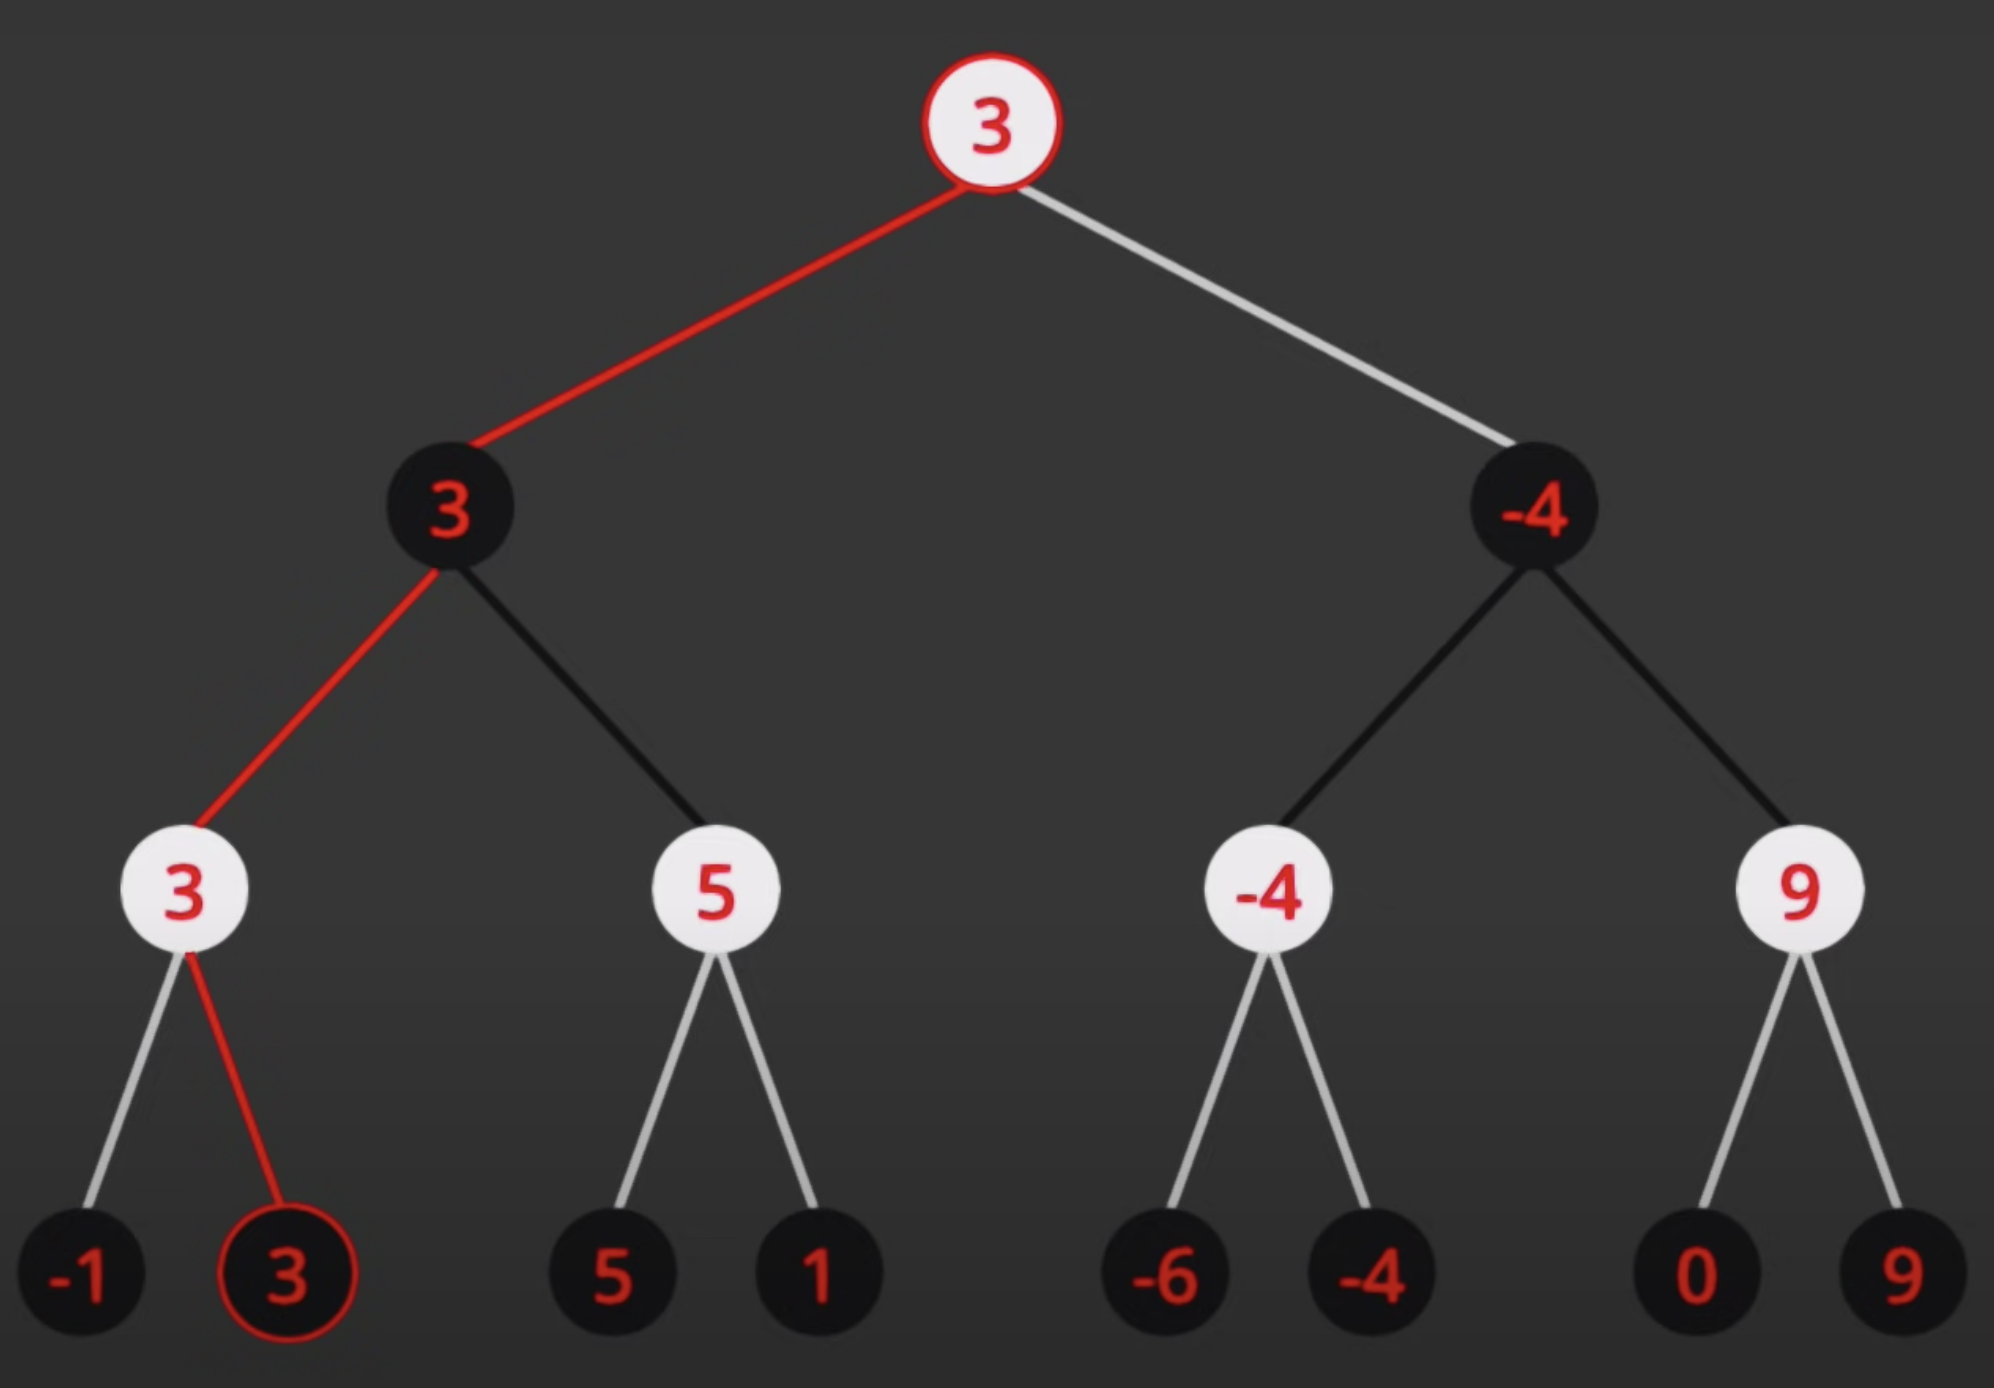
\includegraphics[width=\textwidth]{MM.png}
    \caption{Einfache Visualisierung von Minimax. Weiß: max, schwarz: min}
    \label{fig:minimax}
  \end{minipage}
  \hfill
  \begin{minipage}[b]{0.49\textwidth}
    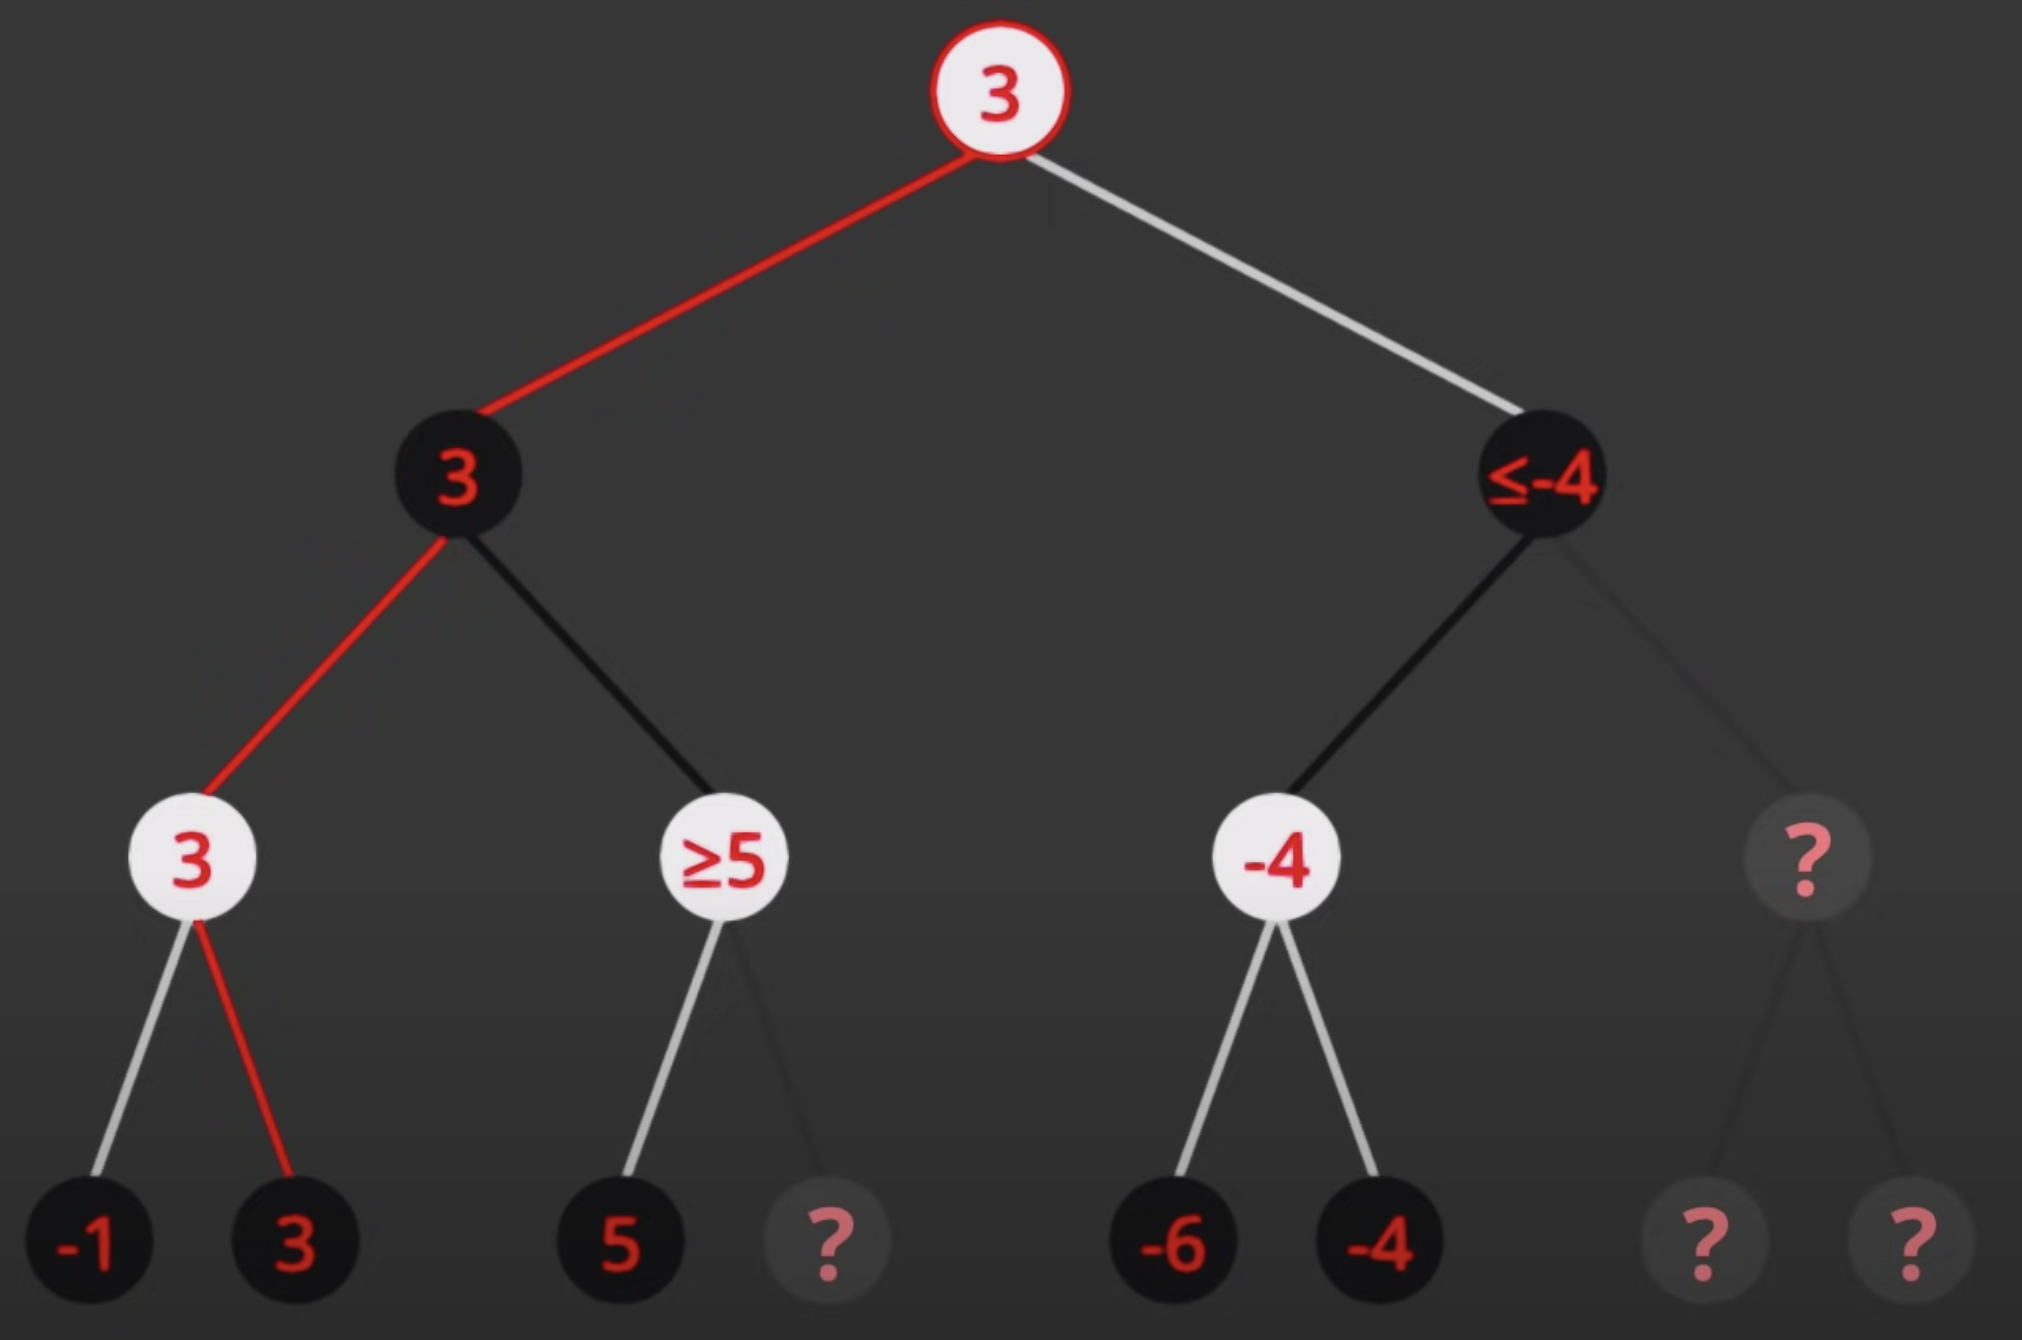
\includegraphics[width=\textwidth]{ABP.png}
    \caption{Der gleiche Suchbaum, mit Alpha-Beta-Pruning}
    \label{fig:alphabeta}
  \end{minipage}
\end{figure}
\subsubsection{Zugsortierung}
Um die Anzahl der abgeschnittenen Zweige bei der Alpha-Beta-Suche zu maximieren, habe ich einen Zug Sortier-Algorithmus entwickelt. Dafür wird an jedem Knoten die Priorität jedes Zuges $a$ anhand des Wertes der sich bewegenden Figur $f$ und ggf. einer geschlagenen Figur $c$ bestimmt:
\[v_a = c_a * m - f_a\]
Hierbei ist $m$ eine Konstante, welche die Gewichtung des geschlagenen Figurenwertes kontrolliert. Ich fand heraus, dass die meisten Zweige abgeschnitten werden konnten, wenn $m$ auf den höchsten Wert aller Figuren besitzt, sodass selbst das Schlagen schlechter Figuren mit starken Figuren Vorrang über nicht-schlagende Züge hat.
So wird z.B. ein Turm-schlägt-Bauern Zug vor einem Bauer-schlägt-Turm Zug erforscht, welcher wiederum Vorrang vor einem normalen Bauer-Zug hat.
\subsubsection{Multiprocessing und Parallelismus}
Um die Performance zu verbessern, verteilte ich den Algorithmus mit dem Multiprocessing Modul auf mehrere Prozessor-Kerne und konnte somit in acht Sekunden bis zu fünf Züge in die Zunkunft (\textit{133 Millionen} Positionen) suchen. 
\begin{figure}
  \centering
  \begin{minipage}{0.49\textwidth}
    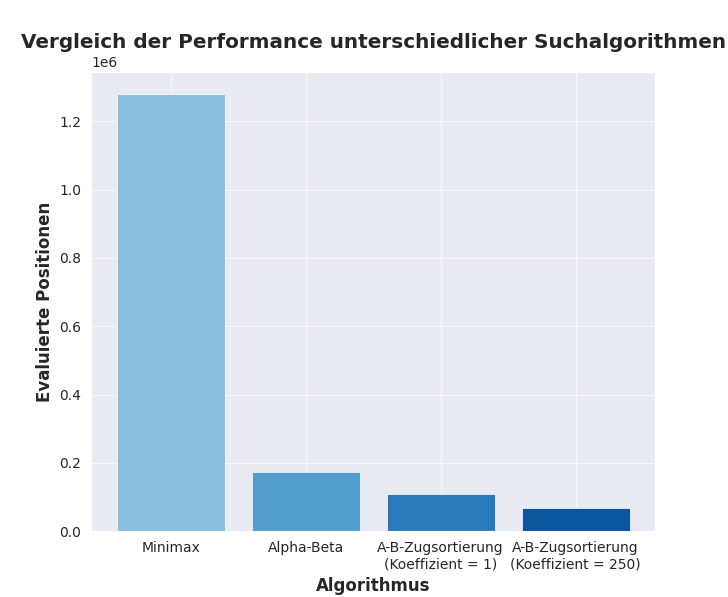
\includegraphics[width=\textwidth]{comp.png}
    \caption{Performance-Vergleich verschiedener Algorithmen}
    \label{fig:algcomp}
  \end{minipage}
  \hfill
  \begin{minipage}{0.4\textwidth}
    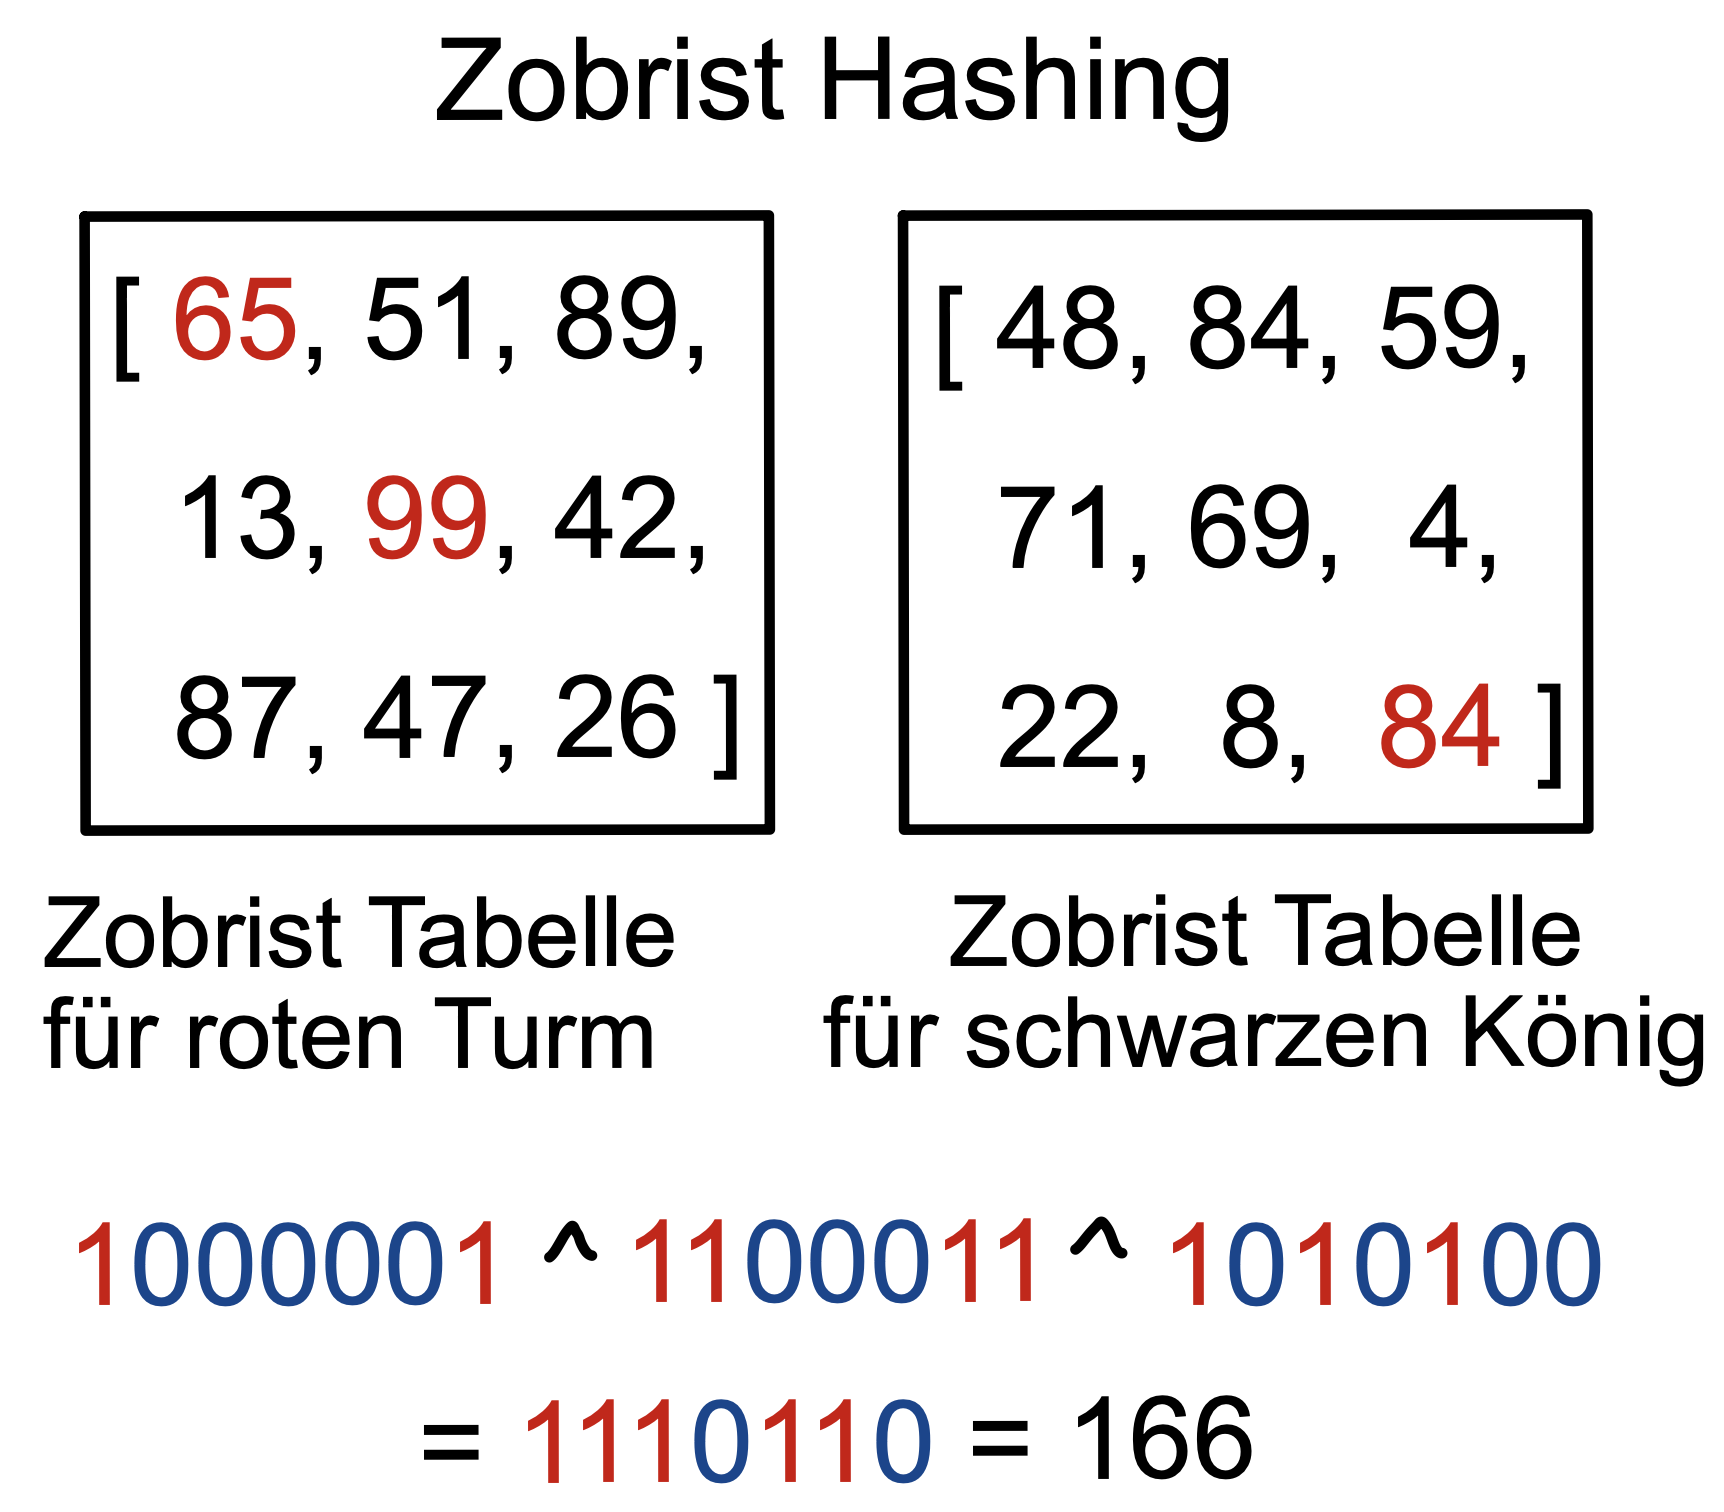
\includegraphics[width=\textwidth]{Zobrist hashing vis.png}
    \caption{Simplifizierte Zobrist Hashing Visualisierung (Bezug auf \ref{fig:repr})}
    \label{fig:zobristvis}
  \end{minipage}
\end{figure}





\subsubsection{Zobrist-Hashing und LaZo}
\textit{Zobrist-Hashing} ermöglicht die effiziente Kodierung (en. hashing) eines Spielzustandes für Spiele wie Xiangqi. Diese kann z.B. genutzt werden, um effizient Positionen zu überspringen, die zu überspring

Es wird dafür vorerst eine Zobrist Tabelle erstellt. Diese besteht aus Zufallszahlen für jede Farbe, jede Figur und jedes Feld und abstrahiert somit Merkmale des Bretts (Positionen der Figuren). Repräsentiert wird sie als dreidimensionales numpy-array bestehend aus 64-Bit ganzen Zahlen. 

Jeder Spielzustand wird durch die bitweise XOR-Verkettung (Kontravalenz) der Zufallszahlen in der Tabelle und der sich bewegenden Seite dargestellt.

Hierbei entwarf ich ein Konzept, welches ich \textit{Lazy-Zobrist (LaZo) }nenne, das die Performance um bis zu 1600\% erhöht \ref{fig:zobrist_perf}. Was zu dieser Performancesteigerung führt LaZo auf Veränderungen anstatt auf Merkmale fokussiert. Da sich nach jedem Zug der Zustand von nur maximal zwei Figuren (wenn eine geschlagen wird) und die sich bewegende Seite ändert, muss der Hash-Wert nicht jedes mal neu generiert werden. Stattdessen wird der bereits existierende Wert modifiziert \ref{fig:method} und sorgt für ein identisches Resultat mit deutlich weniger Berechnungen. Dies funktioniert vor allem dank der Eigenschaft von Kontravalenzen, frühere Operationen Rückgängig machen zu können. 

Aufgrund der immensen Anzahl an möglichen Kombinationen (64-Bit $\rightarrow$ $2^{64}$) sind Hash-Kollisionen (mehrere Eingabedaten erzeugen den gleichen Hash-Wert) sehr selten, was Zobrist-Hashing zu einer sehr zuverlässigen Methode macht.

\begin{figure}
  \centering
  \begin{minipage}{0.49\textwidth}
    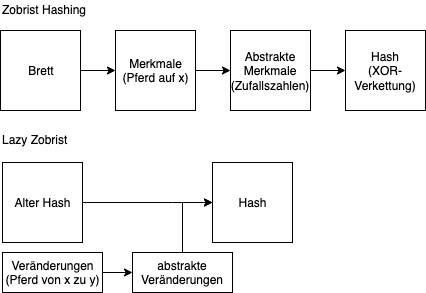
\includegraphics[width=\textwidth]{Zobrist vs. Lazo.png}
    \caption{Zobrist Hashing vs. Lazy-Zobrist}
    \label{fig:method}
  \end{minipage}
  \hfill
  \begin{minipage}{0.49\textwidth}
    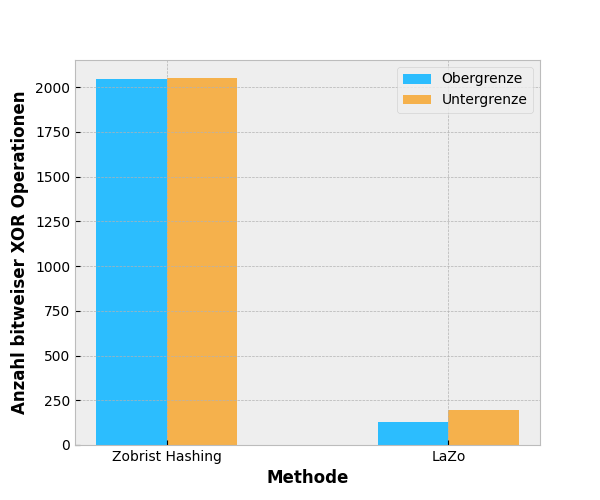
\includegraphics[width=\textwidth]{Zobrist comparison.png}
    \caption{Performance Zobrist Hashing vs. Lazy-Zobrist}
    \label{fig:zobrist_perf}
  \end{minipage}
\end{figure}

\subsection{Autodidaktisches Reinforcement Learning}
Um auf viele weitere domänenspezifische Optimierungen und menschlicher Arbeit verzichten zu können, machte ich es mir zum Ziel, einen weiteren großen Schritt zu gehen und dem Computer das Lernen zu Lehren. Da keine riesigen Datenbanken an Trainingsdaten für Xiangqi-KIs existieren, muss der Algorithmus selber in der Lage sein, diese Trainingsdaten zu generieren. Zur Verfügung stehende Mittel sind dabei nur die Spielregeln. In anderen Worten: Etwa wie wir Menschen soll ein Deep Convolutional Neural Network durch eine Vielzahl von Spielen gegen sich selbst, tabula rasa, Xiangqi meistern. Hierfür hat Deepmind 2017 einen Forschungsbericht über AlphaZero veröffentlicht, in dem die grundsätzliche Idee beschrieben wurde. Es ist aber zu beachten, dass die Architektur und genauere Informationen zum Trainings-Algorithmus von AlphaZero geheim sind und darüber hinaus anzunehmen ist, dass normale Hardware sie bei weitem nicht handhaben kann. Dieser Teil des Projekts erforderte mehrere Monate an Recherche und Kopfzerbrechen.

\begin{figure}
\centering
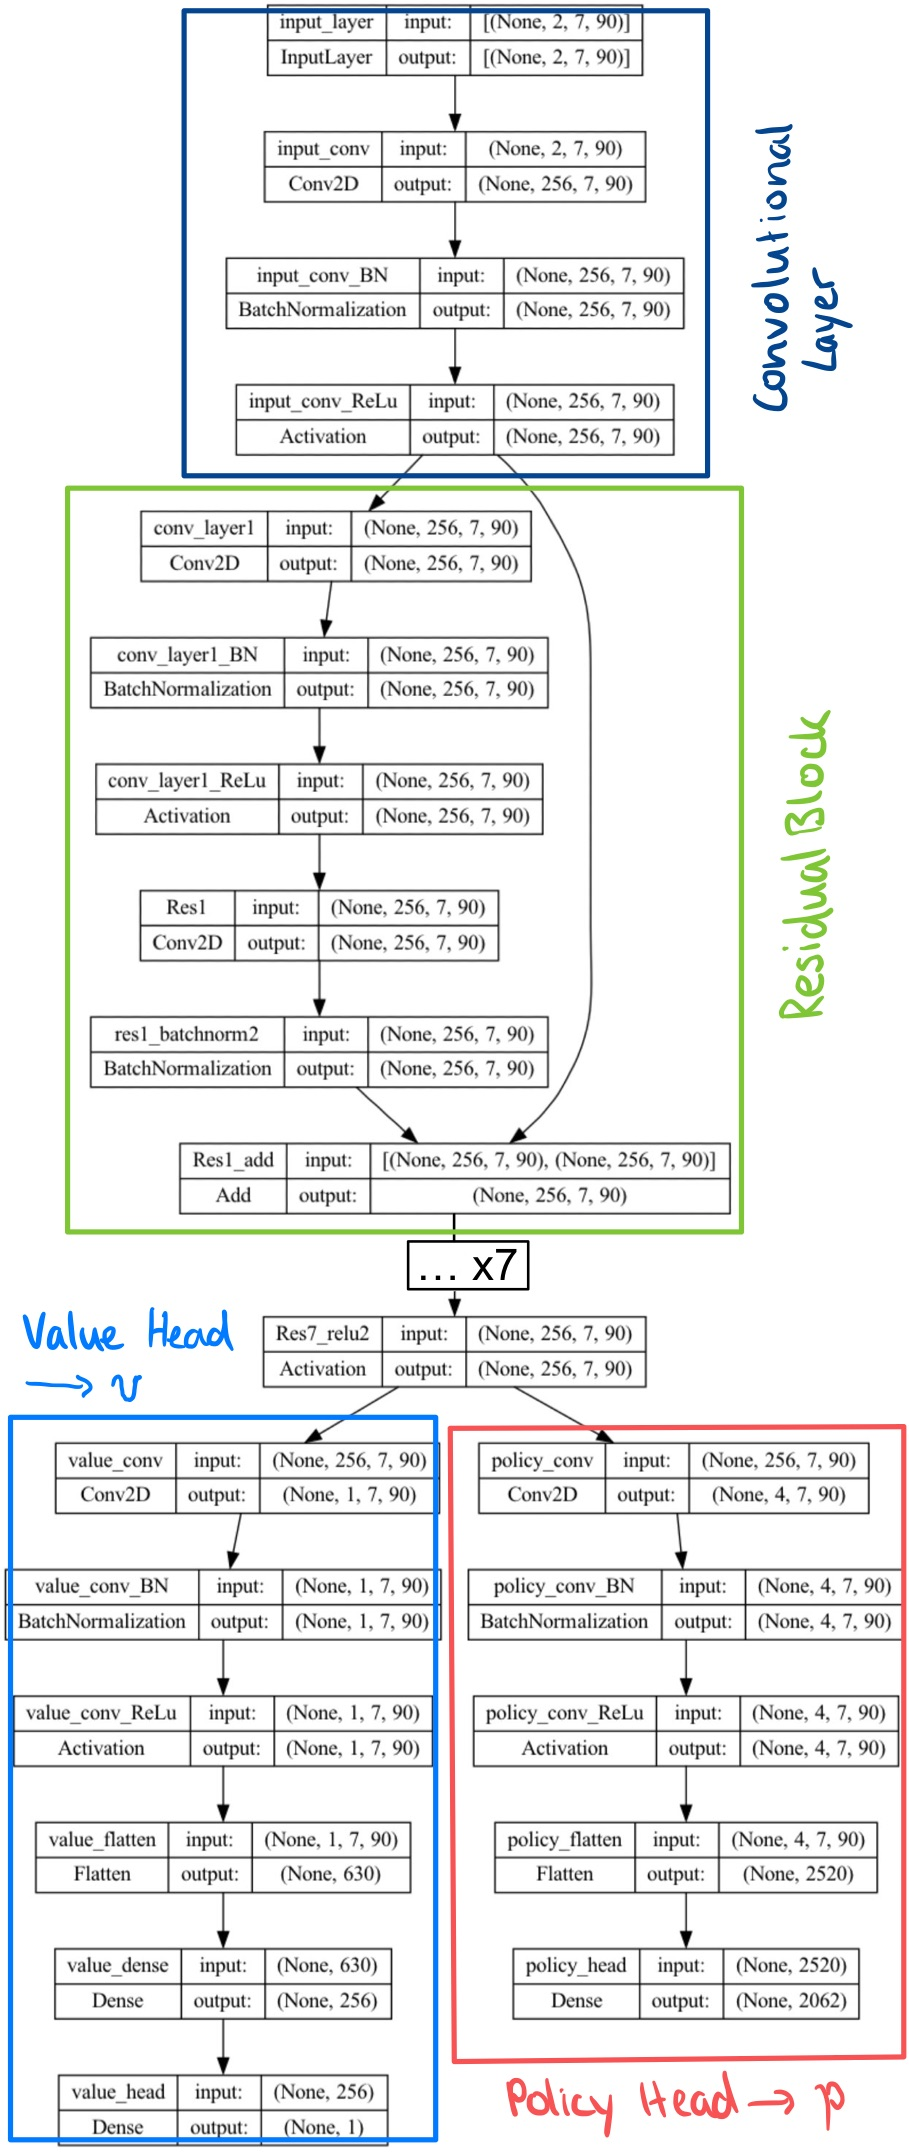
\includegraphics[width={0.63\textwidth}]{model.jpg}
\caption{Neuronales Netzwerk visualisiert}
\label{fig:model}
\end{figure}

\subsubsection{Modellarchitektur}
Ich entwarf ein Deep Convolutional Residual Neural Network mit tensorflow und keras, welches für normale Hardware gut geeignet ist. Hier war es wichtig, die Architektur möglichst klein zu halten, gleichzeitig aber so groß zu lassen, dass es lernfähig ist. Mathematisch sieht es wiefolgt aus:
\[(p, v) =  f_\theta(s)\]Eingabe ist die Brettposition $s$, Ausgabe ein Vektor einer Wahrscheinlichkeitsverteilung $p$ über alle Züge in der Action Space und ein Skalar $v$ zwischen -1 (Niederlage) und 1 (Sieg), der das erwartete Ergebnis von Position $s$ schätzt. Das Netzwerk lernt die optimalen Parameter $\theta$. Es lernt in anderen Worten also, wie gut bestimmte Züge in einer bestimmten Position sind und den Wert der Position selbst zu schätzen. 
Meine Architektur besteht aus zwei Hauptkomponenten:
\begin{enumerate}
\item Ein Convolutional Layer. Diese sind generell besonders gut für Erkennung räumlicher Hierarchien und Muster, ähnlich wie das menschliche visuelle System. Der Convolutional Layer nimmt den aktuellen Brettzustand als Eingabe und gibt eine Reihe von Merkmalen aus, die das Brett repräsentieren.
\item Ein Multi-Layer Perceptron (MLP), das die Ausgabe vom Concvolutional Layer als Eingabe nimmt und neben dem geschätzten Wert des Spielzustandes $v$ eine Wahrscheinlichkeitsverteilung $p$ über alle möglichen Züge ausgibt. Das MLP besteht aus sieben Residual Layers, einem \textit{value head} (für den Wert $v$) und einem \textit{policy head} (für die Wahrscheinlichkeitsverteilung $p$). 
\end{enumerate}
Residual-Schichten ermöglichen es dem Netzwerk statt der Ausgabe den Residual, also den Unterschied zwischen Eingabe und gewünschter Ausgabe, zu lernen. Dadurch wird das Problem des verschwindenden Gradienten behoben. Residual-Schichten erleichtern auch das Training sehr tiefer Netzwerke, da sie es ermöglichen, neue Schichten hinzuzufügen, ohne die Leistung zu verschlechtern. 
\subsubsection{Monte-Carlo Tree Search (MCTS)}
Wie in der Alpha-Beta-Suche repräsentiert jeder Knoten im Such-Baum einen Spielzustand. Ein Kante zum untergeordneten Knoten kann nur bestehen, wenn der Zug erlaubt ist. 
Die Funktionsweise wird aus gleichen Gründen wie beim Zuggenerator abstrahiert. Wichtig ist, dass MCTS auf der Idee basiert, den menschlichen Gedankenverlauf zu simulieren und dass die Suche eine neue, informierte und somit genauere Wahrscheinlichkeitsverteilung $\pi$ mithilfe des aktuellen CNN $f_\theta$  generiert, welche dann genutzt werden, um die Parameter $\theta$ anzupassen.

Der Algorithmus besteht aus vier Schritten: Auswahl, Erweiterung, Simulation und Backpropagation.
\begin{enumerate}

\item Auswahl: Im ersten Schritt wird der Algorithmus durch den aktuellen Zustand des Spiels navigieren und den Zug auswählen, der die höchste geschätzte Siegchance hat.

\item Erweiterung: Sobald ein Blattknoten erreicht ist, wird dieser mit untergeordneten Knoten erweitert. die zukünftige Zustände des Spiels repräsentieren.

\item Simulation: Der Algorithmus bestimmt dann die Wahrscheinlichkeit, dass der ausgewählte Zug zum Sieg führt. Hierfür wird die Wert-Ausgabe $v$ vom Neuronalen Netzwerk genutzt.

\item Backpropagation: Schließlich werden die Ergebnisse der Simulationen zurückpropagiert, um die geschätzte Siegchance für jeden besuchten Knoten im Entscheidungsbaum zu aktualisieren.
\end{enumerate}

\subsubsection{Perspektivische Anpassungen}
Nachdem ich das Grundprinzip des selbstlernenden Algorithmus  implementiert hatte, bekam ich die Idee, die Bitboards und Züge immer an die Perspektive eines  Spielers anzupassen.
Dadurch wird die Anzahl der Labels, also der Größe der CNN-Ausgabe verringert, da einige Züge nach perspektivischer Anpassung äquivalent sind, z.B. (89, 71) und (0, 18). Diese Methode ist menschennaher und sorgt für reduzierte Modellkomplexität, schnelleres Lernen und erhöhte Performance. Viel wichtiger ist aber, dass so allgemeinere Muster erkannt, standardisierte Trainingsdaten gesammelt und Verwirrung beim Training durch unterschiedliche Wertungen perspektivisch äquivalenter Züge vermieden werden können. Denn es ist somit kein “side plane” mehr als Eingabe erforderlich, um die sich bewegende Seite anzugeben und die Eingabe komplett für die Erkennung von Mustern auf dem Brett optimiert ist. Ein weiterer wichtiger Vorteil ist die Augmentation von Trainingsdaten um 200\%, weil für jede Position aus beiden Perspektiven ein Trainingsbeispiel gesammelt werden kann.

\subsubsection{Training}
Traingsdaten werden durch Spiele gegen sich selbst mit MCTS gesammelt. Am Ende jedes Spiels wird jedes Trainingsset mit dem Endergebnis $z$ ergänzt, sodass neben der verbesserten Wahrscheinlichkeitsverteilung $\pi$ auch die Bewertung der Positionen genauer sind. Das Ziel vom Training ist es, die Differenz zwischen vorhergesagtem Ergebnis $v$ und Endergebnis $z$ zu minimieren und die Ähnlichkeit zwischen vorhergesagter Wahrscheinlichkeitsverteilung $p$ und $\pi$ zu maximieren, sodass das Netzwerk $f_\theta$ immer genauere Vorhersagen treffen kann.
Hierfür nutze ich den SGD (Stochastic Gradient Descent) Optimierer und eine Verlust-Funktion $l$, welche mean-squared-error (MSE) für die Ergebnisse und categorical-cross-entropy für die Wahrscheinlichkeitsverteilung nutzt. Mathematisch notiert sieht diese wiefolgt aus:
\[
l = (z - v)^2 - \pi^T \log p + c\lVert \theta \rVert^2
\]
Das $T$ steht für \textit{Transpose}, eine Matrizen-Operation, die benutzt wird, um die Dimensionen für eine Matrizen-Multiplikation anzupassen.
\section{Alpha-Beta-Zero}
Nun habe ich bereits zwei komplett unterschiedliche Algorithmen implementiert.
Alpha-Beta-Zero ist der Teil von Algorithmus, in der ich Alpha-Beta-Suche und den von AlphaZero inspirierten selbstlernenden Reinforcement Learning Algorithmus kombiniere. Hierbei ermittele ich vorerst den ausgewählten Zug beider Algorithmen, $a$ und $b$, und addiere die Evaluation dieser Züge von beiden Such-Algorithmen, um am Ende den Zug mit dem höhsten Wert $V$ auszuwählen.
\[V = max(\pi_a * m + \beta_a, \pi_b * m + \beta_b)\] (Die Evaluationen beider Algorithmen sind $\pi$ für MCTS, $\beta$ für Alpha-Beta-Suche)
Dabei wird der Wert beider Züge laut des MCTS-Algorithmus um $m$ mehr gewichtet, sodass nur bei offensichtlichen Entscheidungsfehlern eine änderung des Zuges vorgenommen wird. Die Entscheidungen der MCTS-Suche werden von einer parallel-ausgeführten Alpha-Beta-Suche kombiniert.

\section{Ergebnisse}
Nach gut einem halben Jahr und unendlich vielen Iterationen von Recherchieren, Nachdenken, Ausprobieren, Scheitern und wieder Recherchieren gelang es mir, erfolgreich eine Xiangqi-KI zu entwickeln, die einen selbstlernenden Algorithmus mit der traditionellen Alpha-Beta-Suche harmonisch ergänzt. 

Ich entwickelte dafür einen domänenspezifisch optimierten Alpha-Beta-Suchalgorithmus und entwarf eine neue Methode, um Zobrist-Hashing um bis zu 1600\% zu verbessern. 

Im Reinforcement Learning Algorithmus konnten reduzierte Modellarchitektur-Komplexität erfolgreich durch neue Optimierungen mithilfe von Perspektivitätsanpassung ausgeglichen werden. Das Training verläuft reibungslos auf einer einzelnen GPU \ref{fig:loss} und die benötigte Hardware konnte von 5000+ TPUs auf einen Laptop reduziert werden, was einer Verbesserung von ca. 500.000\% entspricht.

Die Alpha-Beta-Zero KI schlägt mittlerweile die zweit-beste KI auf Xiangqi.com und hält auch bei dem "Endboss" lange mit.

Mein Zuggenerator ist jeztz die schnellste Python-Implementation weltweit und kann bei Performance-Tests auf meinem Laptop bis zu 108 Millionen Blattknoten pro Sekunde erreichen \ref{fig:perft}. Diese Performance-Tests (perft) werden durchgeführt, um die Leistung des Zuggenerators zu ermitteln und seine Genauigkeit durch den Vergleich mit dem Konsens anderer Programme zu überprüfen. Diese stimmen zu 100\% überein. 

\begin{figure}
  \centering
  \begin{minipage}{0.45\textwidth}
    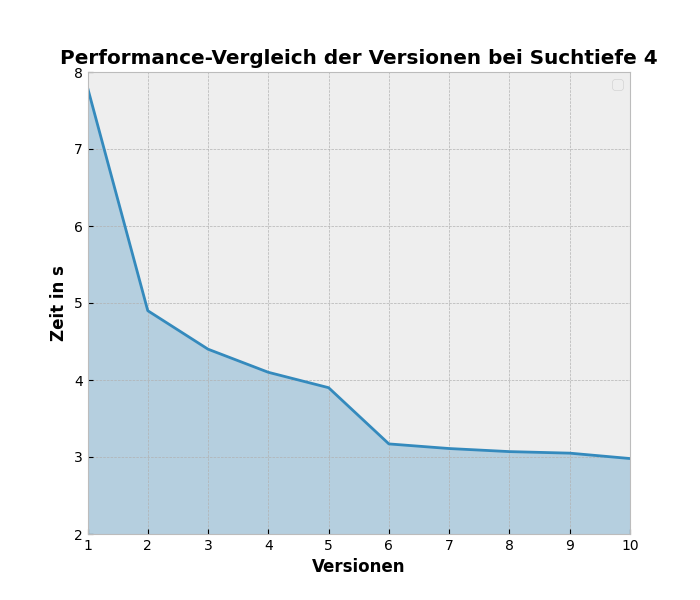
\includegraphics[width=\textwidth]{Perft.png}
    \caption{benötigte Zeit, um 324 Millionen Positionen zu erreichen}
    \label{fig:perft}
  \end{minipage}
  \hfill
  \begin{minipage}{0.54\textwidth}
  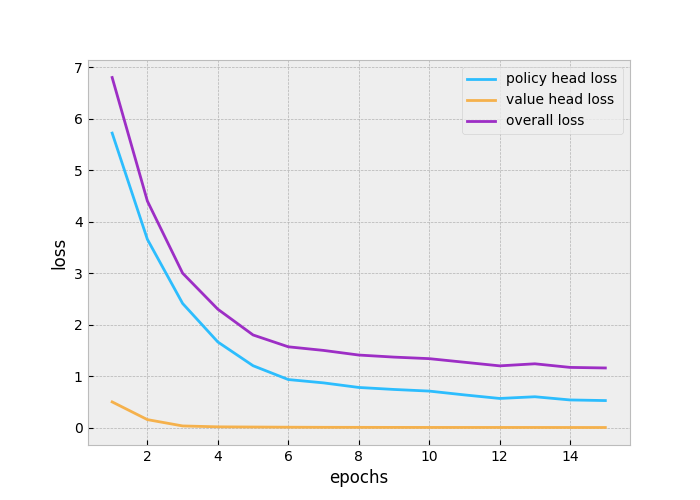
\includegraphics[width={\textwidth}]{loss.png}
  \caption{Die Loss-Werte im Laufe von 15 Trainings-Epochen mit Daten von drei Spielen gegen sich selbst}
  \label{fig:loss}
  \end{minipage}
\end{figure}

\section{Ausblick}
Das Projekt befindet sich derzeit immer noch im Entwicklungsstadium. Der nächste Schritt ist die Evaluation meiner Alpha-Beta-Zero Methode, etwa durch das Entwickeln eines Elo Systems. So kann die Spielstärke der KI gemessen und seine Entwicklung analysiert werden, damit ich anschließend die Hyperparameter für den Trainingsprozess optimieren kann.
Der Zuggenerator ist nach zahlreichen Optimierungen zwar schon hochperformant, besitzt aber noch weiteres Potenzial für Steigerungen der Performance durch Just-in-time-Kompilierung mithilfe von Bibliotheken wie numba (dann wäre es aber natürlich nicht mehr pures Python). Auch die Alpha-Beta-Suche kann weiter verbessert werden, etwa mit Methoden wie iterative deepening, transposition tables und der Optimierung vom Parallelismus.

Ein weiterer Schritt, den man zukünftig gehen könnte, ist die Modifizierung eines echten Bretts, sodass die KI mithilfe eines Microcontrollers ein eingebautes mechanisches Kontrukt unter dem Brett steuern kann, um die Entscheidungen der KI in echte Züge auf einem physischen Brett zu übertragen.

\section{Zusammenfassung}
Zusammengefasst konnte ich die benötigte Hardware innovativer Algorithmen um ca. $500.000\%$ reduzieren, indem ich diesen mit einem hochoptimierten traditionellen Suchalgorithmus ergänzte. Um dies zu ermöglichen, habe ich neue Konzepte entwickelt und Algorithmen entworfen. Dafür musste ich nicht nur zahlreiche neue mathematische Konzepte verstehen sondern auch mein algorithmisches Denken an die Grenzen bringen. 

Ich habe realisiert, dass neue Konzepte oft durch die Kombination von Neu und Alt, durch die Erweiterung von innovativen Konzepten und traditionell anerkannten Methoden, entstehen.

Ich lernte auch, dass diese neuen Konzepte nur durch kritisches Hinterfragen und intensiver Beschäftigung mit den herkömmlichen Methoden entsteht und oft sehr viel Mut und eine Bereitschaft zum Scheitern erfordert. Meine Perspektive zu Bugs und ungeplantem Verhalten des Programms änderte sich und ich fing an sie nicht als Scheitern, sondern als Versuche zu sehen.  

Es war ein langer Prozess vom wiederholten Kopfzerbrechen und Scheitern, der mir beibrachte, dass das Verstehen von komplexen Themen manchmal vielleicht gar nicht so unmöglich ist wie es scheint. Mit etwas Bescheidenheit, der Akzeptanz des eigenen Unwissens und sehr viel Offenheit zum Lernen kann man diese Konzepte nicht nur verstehen und umsetzen, sondern auch erweitern, auf Ihnen aufbauen, vielleicht anderen Menschen helfen und auf dem Weg zu einem besseren Informatiker werden.

\section{Quellen- und Literaturverzeichnis}

\url{https://github.com/Simuschlatz/CheapChess}, 15.01.23, Simon Ma, CheapChess Quellcode für detaillierte Beschreibungen der angewandten Methoden
\\
\url{https://www.chessprogramming.org/Main_Page}, 15.01.23, 
Chessprogramming Wiki, Wikipedia für Schachprogrammierung
\\
\url{https://en.wikipedia.org/wiki/Monte_Carlo_tree_search}, 15.01.23, Wikipedia, Monte-Carlo-Tree-Search
\\
\url{https://de.wikipedia.org/wiki/Xiangqi}, 15.01.21, Wikipedia, Xiangqi
\\
\url{https://www.xiangqi.com/}, 15.01.23, Xiangqi.com, Play Chinese Chess For Free on the \#1 Xiangqi Site!
\\
\url{https://www.deepmind.com/}, 15.01.23, Deepmind, Tocherfirma von Google
\\
\url{https://arxiv.org/abs/1712.01815}, Deepmind, Mastering Chess and Shogi by Self-Play with a General Reinforcement Learning Algorithm
\\
\url{https://www.youtube.com/c/SebastianLague}, 15.01.23, Sebastian Lague
\\
\url{https://www.youtube.com/watch?v=l-hh51ncgDI}, 21.08.22, Sebastian Lague, Algorithms Explained – minimax and alpha-beta pruning

\end{document}